% main_blind_review.tex
% GTAC 2026 double-blind submission

\documentclass[blind]{gtac}

\usepackage{cite}
\usepackage{xcolor}
\usepackage{booktabs}
\usepackage{tikz}
\usetikzlibrary{arrows.meta,positioning}
\usepackage[colorlinks=true, linkcolor=blue, urlcolor=blue, citecolor=blue]{hyperref}
\Urlmuskip=0mu plus 1mu\relax % allow long URLs in references to break

\SetWatermarkScale{0.3}
\SetWatermarkAngle{30}
\SetWatermarkColor{gray!20}

\title{Owning the Inference Layer of the Voice AI Stack: A ROCm Characterization and a Path to Close the Streaming-ASR and Embedding Gaps\subtitle{Submitted Anonymously for Double-Blind Review}}

\author{Anonymous}

\begin{document}

\maketitle

\pagestyle{fancy}
\fancyhf{}
\cfoot{\thepage}
\renewcommand{\headrulewidth}{0pt}
\chead{{\sffamily\textcolor{red}{\fontsize{10}{12}\selectfont\textbf{DO NOT FORWARD -- FOR GTAC'26 REVIEW COMMITTEE ONLY}}}}
\thispagestyle{fancy}

\begin{abstract}
Conversational voice AI has crossed from novelty to production infrastructure: median end-to-end response latency fell from 1{,}200\,ms in 2024 to 680\,ms in 2026, and the AI voice-agent market is projected to grow from \$2.4B (2024) to \$47.5B (2034) at a 35\% CAGR. Unlike model \emph{training}, a deployed voice agent is an \emph{inference} workload that runs continuously, and at scale its dominant operating cost is GPU compute for three layers: speech recognition, language modeling, and speech synthesis. We characterize the five-layer voice pipeline as a latency- and cost-budgeted system and benchmark its compute-bearing layers on AMD Instinct MI300X relative to NVIDIA H100. We find a structural AMD advantage on the two heaviest layers---a 34\% lower cost-per-token for 70B-class large language model (LLM) inference and single-GPU fit (192\,GB HBM3) for models that otherwise require two H100s---while pure-PyTorch text-to-speech (TTS) runs unmodified on ROCm. We then isolate the two concrete software gaps that block a fully ROCm-native deployment---streaming ASR containers and HuggingFace Text-Embeddings-Inference (TEI) for retrieval-augmented agents---and propose a bounded engineering plan to close them. We quantify the resulting opportunity: a 1M-minute/month deployment saves on the order of \$84K/month on LLM inference alone, and on-premise, data-residency-constrained markets (e.g., India BFSI under the DPDP Act) map directly onto AMD's CapEx advantage. The value to AMD is a defensible inference foothold at the cost- and compliance-sensitive end of a rapidly standardizing stack.
\end{abstract}

\keywords{LLM inference, ROCm, MI300X, automatic speech recognition, text-to-speech, retrieval-augmented generation, total cost of ownership, on-premise inference, Ryzen AI NPU.}

\section{Introduction}
Voice agents now answer phones, qualify leads, triage patients, and run collections at a unit cost (\texttt{\textasciitilde}\$0.40/call) that is one to two orders of magnitude below a human agent (\$7--\$12/call)~\cite{assemblyai_2026,grandview}. The economics are compelling enough that 80\% of customer-service organizations plan a voice AI deployment, and production deployments grew 340\% year-over-year across 500+ organizations~\cite{assemblyai_2026}.

A point that is easy to miss in the excitement over training mega-clusters is that a voice agent in production is a \emph{steady-state inference machine}. It does not train; it transcribes, reasons, and speaks, 24 hours a day. At a million minutes per month its bill is dominated not by API subscriptions but by the GPU cycles consumed in three layers of a fixed pipeline. This reframing matters for AMD: the inference layer is where ROCm is already competitive, where VRAM capacity is a structural lever, and where the buyer is most cost-sensitive.

This paper makes three contributions. First, we model the voice pipeline as a latency- and cost-budgeted system and identify which layers actually bear compute (Section~\ref{sec:pipeline}). Second, we benchmark the compute-bearing layers on MI300X versus H100 and quantify where AMD wins today and where it does not (Section~\ref{sec:bench}). Third, and most novel, we isolate the two specific ROCm ecosystem gaps that prevent a fully AMD-native voice deployment and lay out a bounded plan to close them, then size the business impact (Sections~\ref{sec:gaps}--\ref{sec:impact}). The paper is deliberately self-contained so a future reader can reconstruct both the 2026 stack and the rationale for AMD's positioning.

\section{The Voice AI Pipeline as a Budgeted System}
\label{sec:pipeline}
A natural-feeling conversation requires the entire round trip---from the moment a caller stops speaking to the first synthesized syllable of the reply---to complete within roughly half a second. The 2026 production median is 680\,ms and the emerging bar is sub-500\,ms, which is especially tight on Indian cellular networks that add \texttt{\textasciitilde}50\,ms over fiber~\cite{assemblyai_stack}. That budget is spent across five layers (Figure~\ref{fig:pipe}).

\begin{figure}[t]
\centering
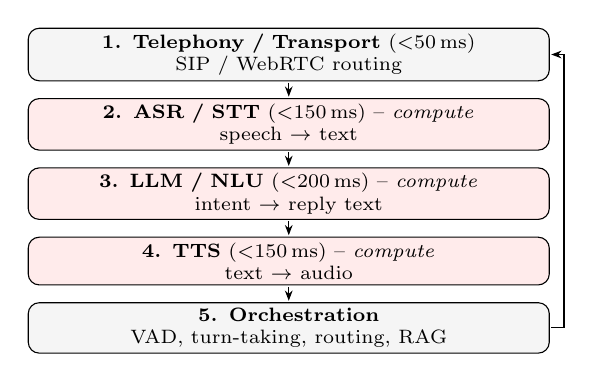
\begin{tikzpicture}[
  font=\scriptsize,
  box/.style={draw, rounded corners, align=center, text width=2.55in, minimum height=2.6ex, inner sep=2pt},
  comp/.style={box, fill=red!8},
  light/.style={box, fill=gray!8},
  arr/.style={-{Stealth[length=1.3mm]}, shorten >=0.5pt, shorten <=0.5pt}
]
\node[light] (tel) {\textbf{1. Telephony / Transport} ($<$50\,ms)\\ SIP / WebRTC routing};
\node[comp, below=1.4ex of tel] (asr) {\textbf{2. ASR / STT} ($<$150\,ms) -- \emph{compute}\\ speech $\rightarrow$ text};
\node[comp, below=1.4ex of asr] (llm) {\textbf{3. LLM / NLU} ($<$200\,ms) -- \emph{compute}\\ intent $\rightarrow$ reply text};
\node[comp, below=1.4ex of llm] (tts) {\textbf{4. TTS} ($<$150\,ms) -- \emph{compute}\\ text $\rightarrow$ audio};
\node[light, below=1.4ex of tts] (orc) {\textbf{5. Orchestration}\\ VAD, turn-taking, routing, RAG};
\draw[arr] (tel) -- (asr);
\draw[arr] (asr) -- (llm);
\draw[arr] (llm) -- (tts);
\draw[arr] (tts) -- (orc);
\draw[arr] (orc.east) -- ++(0.18,0) |- (tel.east);
\end{tikzpicture}
\caption{The five-layer voice pipeline with per-layer latency budget. The three shaded layers (ASR, LLM, TTS) are the GPU-compute-bearing layers and the locus of AMD's opportunity; orchestration closes the loop.}
\label{fig:pipe}
\end{figure}

Two layers (telephony and orchestration) are I/O- and control-bound and carry little GPU cost. The three middle layers are where the money and the milliseconds go. Counterintuitively, \emph{LLM inference is the cheapest of the three per minute but the most latency-critical}: it must emit its first token in under 200\,ms, which favors smaller, faster models (Llama 3.1 8B, Mistral 7B) and time-to-first-token optimization over raw throughput. TTS is the \emph{hidden budget killer}---premium hosted synthesis (\$0.10--\$0.30/min) can exceed ASR and LLM combined---which is precisely why self-hosted, GPU-resident TTS is economically attractive and why the GPU choice matters~\cite{bentoml_tts}.

\section{ROCm Characterization of the Compute Layers}
\label{sec:bench}
We assess each compute layer on MI300X (192\,GB HBM3) against H100 SXM5 (80\,GB), using 2026 cloud price points and public throughput figures~\cite{spheron_rocm,vllm_rocm,mlperf6}. The question is not abstract performance but \emph{cost per unit of conversation} and \emph{whether the model fits}.

\subsection{LLM Layer: Cost-per-Token and VRAM Fit}
For a Llama 3.1 70B serving workload, Table~\ref{tab:llm} shows MI300X delivering comparable throughput at substantially lower hourly cost, yielding a 34\% lower cost-per-million-tokens. A voice deployment handling 1M minutes/month generates on the order of 6B tokens/month; the per-token delta compounds to roughly \textbf{\$84K/month} in inference savings at that scale.

\begin{table}[t]
\centering
\caption{LLM inference for Llama 3.1 70B (2026 figures).}
\label{tab:llm}
\footnotesize
\begin{tabular}{@{}lcc@{}}
\toprule
Dimension & MI300X & H100 SXM5 \\
\midrule
VRAM & \textbf{192\,GB} HBM3 & 80\,GB HBM3e \\
On-demand price & \$1.50--2.50/hr & \$2.90/hr \\
Throughput (tok/s) & \texttt{\textasciitilde}18{,}000 & \texttt{\textasciitilde}19{,}500 \\
Cost / 1M tokens & \textbf{\$0.027} & \$0.041 \\
70B fits on 1 GPU? & \textbf{Yes} & No (needs 2) \\
\bottomrule
\end{tabular}
\end{table}

The VRAM result is structural rather than incremental. A 70B-class model---common for high-quality enterprise agents---requires two H100s (160\,GB combined) but fits on a single MI300X. This halves node count, removes the NVLink/interconnect tax, and simplifies the serving topology. On MLPerf Inference v6.0, MI355X (288\,GB HBM3e) landed within single-digit percentage points of B200 on server inference, confirming the gap is closing at the high end as well~\cite{mlperf6}.

\subsection{TTS Layer: Pure PyTorch Runs Unmodified}
The leading self-hostable TTS models---Kokoro (82M, Apache 2.0), Chatterbox, and Coqui XTTS-v2---are pure PyTorch and run on ROCm without source changes, because HIP transparently maps the CUDA calls~\cite{bentoml_tts}. For any operator self-hosting TTS to escape per-minute hosted pricing, AMD is already a viable, cost-competitive target with no porting effort.

\subsection{ASR Layer: Batch Works, Streaming Does Not (Yet)}
Batch ASR (Faster-Whisper, distil-whisper, WhisperX) runs well on ROCm. The problem is that all Whisper variants are \emph{batch-only}; a real-time agent needs \emph{streaming} ASR paired with voice-activity detection (VAD), and the streaming ecosystem is built assuming CUDA. This is the first of the two gaps, and we treat it as engineering work, not a silicon limitation, in Section~\ref{sec:gaps}. ASR accuracy is also the layer most exposed to real-world conditions: English real-world word error rate (WER) for Whisper Large-v3 is \texttt{\textasciitilde}10.6\% (versus 2.7\% on clean benchmarks), and 8\,kHz telephony, code-switching, and accents push it materially higher~\cite{whisper_wer,indic_asr}.

\subsection{Compatibility Summary}
Table~\ref{tab:compat} consolidates the per-component ROCm status. The pattern is clear: the two heaviest layers (LLM, TTS) are solved; two narrow but load-bearing pieces (streaming ASR, embeddings) are not.

\begin{table}[t]
\centering
\caption{ROCm support for voice-AI components (2026).}
\label{tab:compat}
\footnotesize
\begin{tabular}{@{}lcl@{}}
\toprule
Component & ROCm & Note \\
\midrule
LLM serving (vLLM, Llama 3.1) & Full & 90--95\% of H100 tput \\
LLM serving (SGLang) & Full & within 5--10\% CUDA \\
TTS: Kokoro, Chatterbox & Full & pure PyTorch \\
TTS: Coqui XTTS-v2 & Partial & works with effort \\
ASR: Faster-Whisper (batch) & Full & real-time needs work \\
ASR: streaming containers & \textbf{Gap} & CUDA-assumed \\
Embeddings: HF TEI & \textbf{Gap} & no ROCm build \\
\bottomrule
\end{tabular}
\end{table}

\section{Closing the Two ROCm Gaps}
\label{sec:gaps}
Both blockers are bounded software problems with high ecosystem leverage; neither requires new silicon.

\textbf{Gap 1 --- Streaming ASR.} Commercial streaming ASR vendors and HuggingFace inference containers default to CUDA, so a real-time, low-latency ASR front-end on AMD currently requires custom integration. \emph{Proposed remediation:} publish and maintain a certified ROCm container that composes Faster-Whisper (batch backbone), Silero VAD (turn boundary detection), and an aggressive chunking/streaming wrapper, targeting sub-300\,ms partial transcripts. A high-value, region-specific extension is to validate a telephony-trained Indic ASR model (e.g., Sarvam-class) on MI300X, since global models lose 15--20 WER points on 8\,kHz Hinglish~\cite{sarvam_asr,indic_asr}. This also mitigates the documented Whisper hallucination failure mode (1--80\% of segments on silence/noise), because VAD gating prevents the model from transcribing non-speech~\cite{facct_whisper}.

\textbf{Gap 2 --- Embeddings for RAG.} Enterprise agents ground their answers in product catalogs, policies, and FAQs via retrieval-augmented generation (RAG), which depends on a text-embeddings service. HuggingFace Text-Embeddings-Inference (TEI) has no ROCm build, leaving a hole in an otherwise AMD-native pipeline. \emph{Proposed remediation:} upstream ROCm support into TEI. This is a contained engineering project whose payoff is disproportionate---it unblocks every RAG-augmented voice agent on AMD and complements the existing ROCm RAG/Ollama voice tutorial~\cite{rocm_voice_rag}.

Where AMD remains genuinely behind is ultra-low-latency single-stream decoding at batch size 1--4, where NVIDIA's Hopper-specific FlashAttention-3 and TensorRT-LLM still lead. AMD's countervailing strength is throughput at batch 64--128 and the ROCm 7.x attention-kernel work that is narrowing the kernel gap~\cite{vllm_rocm}. For voice fleets that aggregate many concurrent calls, throughput is the operative metric.

\section{Cost and Business Impact for AMD}
\label{sec:impact}
\textbf{Per-conversation economics.} The compute-bearing layers can be served end-to-end on AMD today (with the two gaps closed). Combining the 34\% LLM cost advantage with self-hosted ROCm TTS, an operator at 1M minutes/month saves on the order of \$50K--\$100K/year on LLM inference alone, before counting the TTS savings from avoiding \$0.10--\$0.30/min hosted synthesis~\cite{raftlabs_cost}.

Table~\ref{tab:cost} attributes full-stack monthly cost across a 10{,}000-minute workload. The decisive line is TTS: hosted synthesis can reach \$3{,}000/month while a ROCm-resident model costs only GPU time, and it is the single largest swing between the self-hosted and managed columns. This is why owning the GPU layer---not merely the LLM---changes the total cost of ownership.

\begin{table}[t]
\centering
\caption{Full-stack cost per 10{,}000 minutes/month.}
\label{tab:cost}
\footnotesize
\begin{tabular}{@{}lcc@{}}
\toprule
Layer & Self-hosted (ROCm) & Managed cloud \\
\midrule
Telephony & \$35--140 & \$35--140 \\
ASR / STT & \$15--50 & \$43--240 \\
LLM & \$20--150 & \$20--150 \\
TTS & \$20--50 & \$200--3{,}000 \\
GPU / infra & \$200--800 & included \\
\midrule
\textbf{Total} & \textbf{\$290--1{,}190} & \textbf{\$298--3{,}530} \\
\bottomrule
\end{tabular}
\end{table}

\textbf{The on-premise / data-residency wedge.} The cleanest entry is markets where the workload \emph{must} run on-premise. India's Digital Personal Data Protection (DPDP) Act treats call audio as biometric data and constrains cross-border transfer, making cloud-only US-hosted stacks legally risky for banking, financial services, and insurance (BFSI)~\cite{dpdp_checklist,india_guide}. On-premise is then mandatory, and on-premise procurement is decided on CapEx---where AMD's roughly 50\% lower GPU list price for equivalent capability, plus single-GPU fit for large models, is a direct advantage. India hosts the second-largest concentration of voice AI startups globally and a market projected to reach \$1B by 2030 (35.7\% CAGR)~\cite{slator_sarvam,india_guide}; sovereign-AI efforts there deploy on-premise by design and are natural ROCm targets.

\textbf{Edge extension.} For last-mile, single-branch deployments, the Ryzen AI NPU already runs Whisper on-device (BFP16, no CPU/GPU load, audio never leaves the device), extending the same data-residency story from the datacenter to the branch~\cite{amd_ryzen_whisper}.

\section{Conclusions}
A production voice agent is an inference workload, and inference---not training---is where AMD is already competitive in this stack. We characterized the five-layer voice pipeline as a latency- and cost-budgeted system, showed by benchmark that MI300X delivers a 34\% lower cost-per-token and single-GPU fit for 70B-class models while pure-PyTorch TTS runs unmodified on ROCm, and isolated the two narrow gaps---streaming ASR containers and HuggingFace TEI---that stand between AMD and a fully native voice deployment. Both gaps are bounded software efforts with high ecosystem leverage, and we proposed concrete remediations for each.

\textbf{Limitations.} Our LLM and TTS results rest on public throughput and price figures rather than a controlled in-house harness, and we have not yet measured a closed-loop end-to-end latency distribution on an all-ROCm stack; the streaming-ASR remediation is specified but not yet implemented and benchmarked. \textbf{Impact on AMD.} The actionable items are small and self-contained: a certified ROCm streaming-ASR container and upstreamed TEI support would make AMD the default cost- and compliance-optimized platform for voice inference, with the on-premise, data-residency-constrained segment (e.g., India BFSI and sovereign AI) as the natural beachhead before the market standard calcifies around a single vendor.

\begingroup
\let\itshape\upshape
\bibliographystyle{abbrv}
\bibliography{refs}
\endgroup

\end{document}
